\documentclass[12pt, a4paper]{article}
\usepackage[utf8]{inputenc}
\usepackage[english,russian]{babel}
\usepackage[T1, T2A]{fontenc}
\usepackage{graphicx}
\usepackage{epstopdf}
\usepackage{caption, subcaption}
\usepackage{threeparttable}
\usepackage[margin=14pt,font=small,labelsep=endash]{caption}
\captionsetup[figure]{labelformat=simple, labelsep = endash, name = Рисунок}
\captionsetup[table]{name = Таблица, labelsep = endash, justification=raggedright, singlelinecheck=false}
\usepackage{float}
\usepackage{geometry} %способ ручной установки полей
\geometry{top=2cm} %поле сверху
\geometry{bottom=2cm} %поле снизу
\geometry{left=2cm} %поле справа
\geometry{right=2cm} %поле слева
\usepackage{amsmath}
\newcommand\tline[2]{$\underset{\text{#1}}{\text{\underline{\hspace{#2}}}}$}
\newcommand\nameLine[3]{$\underset{\text{#1}}{\text{\underline{\text{#2}\hspace{#3}}}}$}

%opening
\title{}
\author{}

\begin{document}
\begin{titlepage}
		\centering
		{\fontsize{12pt}{5cm}\selectfont \bfseries Министерство образования и науки Российской Федерации} \\ \vspace{0.5cm}
		{\fontsize{7pt}{5cm}\selectfont ФЕДЕРАЛЬНОЕ ГОСУДАРСТВЕННОЕ АВТОНОМНОЕ ОБРАЗОВАТЕЛЬНОЕ УЧРЕЖДЕНИЕ ВЫСШЕГО ПРОФЕССИОНАЛЬНОГО ОБРАЗОВАНИЯ} \\ 
		\vspace{1cm}
		{\fontsize{12pt}{5cm}\selectfont \bfseries САНКТ-ПЕТЕРБУРГСКИЙ УНИВЕРСИТЕТ ИНФОРМАЦИОННЫХ ТЕХНОЛОГИЙ, МЕХАНИКИ И ОПТИКИ} \\ \vspace{1.5cm}

		{\fontsize{14pt}{5cm}\selectfont Кафедра \hspace{1cm} \underline{Систем Управления и Информатики}  \hspace{1cm} Группа \underline{Р3340}} \\ 
		\vspace{2cm}

		{\fontsize{20pt}{5cm}\selectfont \bfseries Лабораторная работа №11} \\
		{\fontsize{20pt}{5cm}\selectfont \bfseries Исследование математической модели пьезоэлектрического исполнительного устройства} \\
		{\fontsize{14pt}{5cm}\selectfont Вариант - 9} \\
		\vspace{1.5cm}

		\flushleft

		{Выполнила \hspace{1,7cm} \nameLine{(фамилия, и.о.)}{Сорокина Т. В.}{6.3cm} (подпись)} \\
		\vspace{2cm}

		{Проверил \hspace{2cm} \tline{(фамилия, и.о.)}{9cm} (подпись)} \\
		\vspace{5cm}

		"\underline{\hspace{0.7cm}}"\hspace{0.2cm}\underline{\hspace{2cm}}\hspace{0.2cm}20\underline{\hspace{0.7cm}}г. \hspace{2cm} Санкт-Петербург, \hspace{2cm} 20\underline{\hspace{0.7cm}}г. \\ \vspace{1cm}

		Работа выполнена с оценкой \hspace{1cm} \underline{\hspace{8cm}} \\ 
		\vspace{1cm}
		Дата защиты "\underline{\hspace{0.7cm}}"\hspace{0.2cm}\underline{\hspace{2cm}}\hspace{0.2cm}20\underline{\hspace{0.7cm}}г.

	\end{titlepage}
%\maketitle
%\begin{abstract}
%\end{abstract}

\paragraph {Цель работы:} изучение математических моделей и исследование характеристик исполнительного устройства, построенного на 
основе пьезоэлектрического двигателя микроперемещений.\\
\textbf{Исходные данные}
\par Типовые конструкции пьезоэлектрических двигателей приведены на рисунке 1.
\begin{figure}[H]
\centering
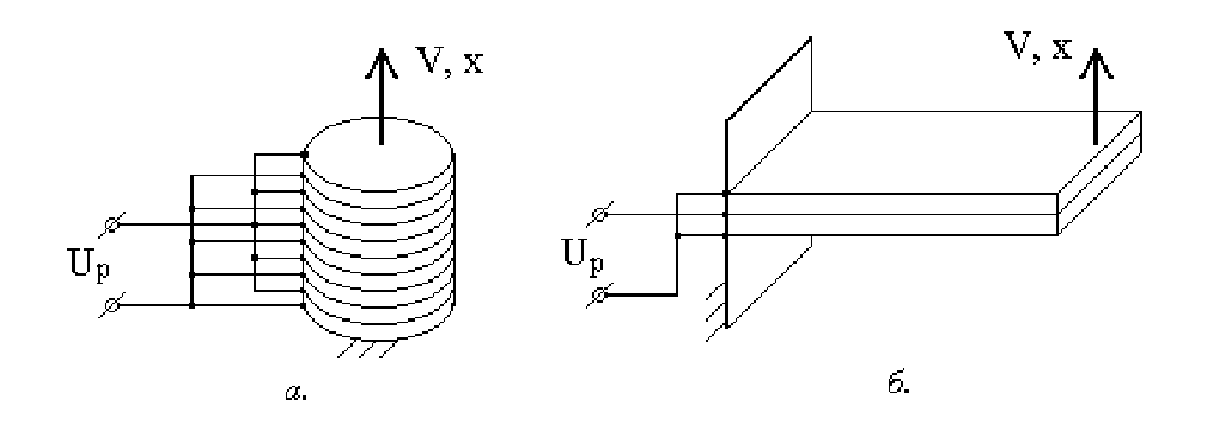
\includegraphics[width=0.7\textwidth]{1/str.eps}
\caption{Составная и биморфная конструкции пьезоэлектрических двигателей}
\end{figure}
В данной лабораторной работе будет исследоваться, биморфный пьезоэлектрический двигатель, изображенный на рисунке 1 под буквой б.
Исходные данные, необходимые для выполнения работы приведены в таблице 1.

\begin{table}[h!]
\centering
\begin{threeparttable}
\caption{Исходные данные}
\renewcommand{\arraystretch}{1.8}
\begin{tabular}{ |c|c|c|c|c|c|c|c|c|} 
 \hline
 $C_{p}$, Н/м & m,кг & $K_{0}$,Н/В & $K_{d}$,Нc/м & $T_{u}$,с & $F_{b}$, Н & $U_{pm}$, В &$U_{m}$, В & $K_{u}$ \\ 
 \hline
  $1.8*10^6$ & 0.01 & 5.2 & $0.7*10^2$ & 0.0002 & 0.9 & 300 & 10 & 30 \\ 
 \hline
\end{tabular}
\end{threeparttable}
\end{table}
\par На рисунке 2 изображена структурная схема пьезоэлектрического исполнительного устройства.
\begin{figure}[H]
\centering
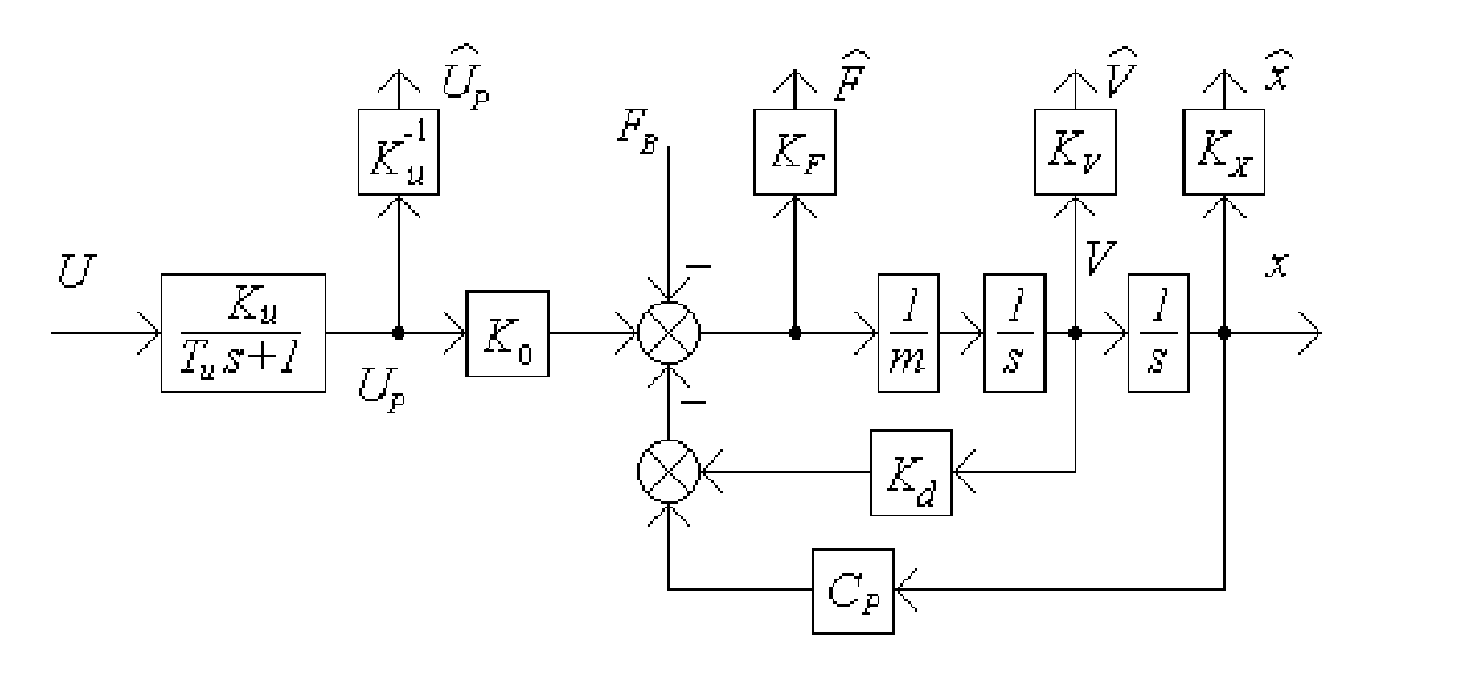
\includegraphics[width=\textwidth]{1/srukt.eps}
\caption{Cтруктурная схема пьезоэлектрического исполнительного устройства}
\end{figure}

\newpage
\begin{center}
\section{Математическое моделирование пьезоэлектрического двигателя}
\end{center} \par
В соответствии со схемой, изображенной на рисунке 2, составим схему моделирования пьезоэлектрического двигателя, которая представлена
на рисунке 3.
\begin{figure}[H]
\centering
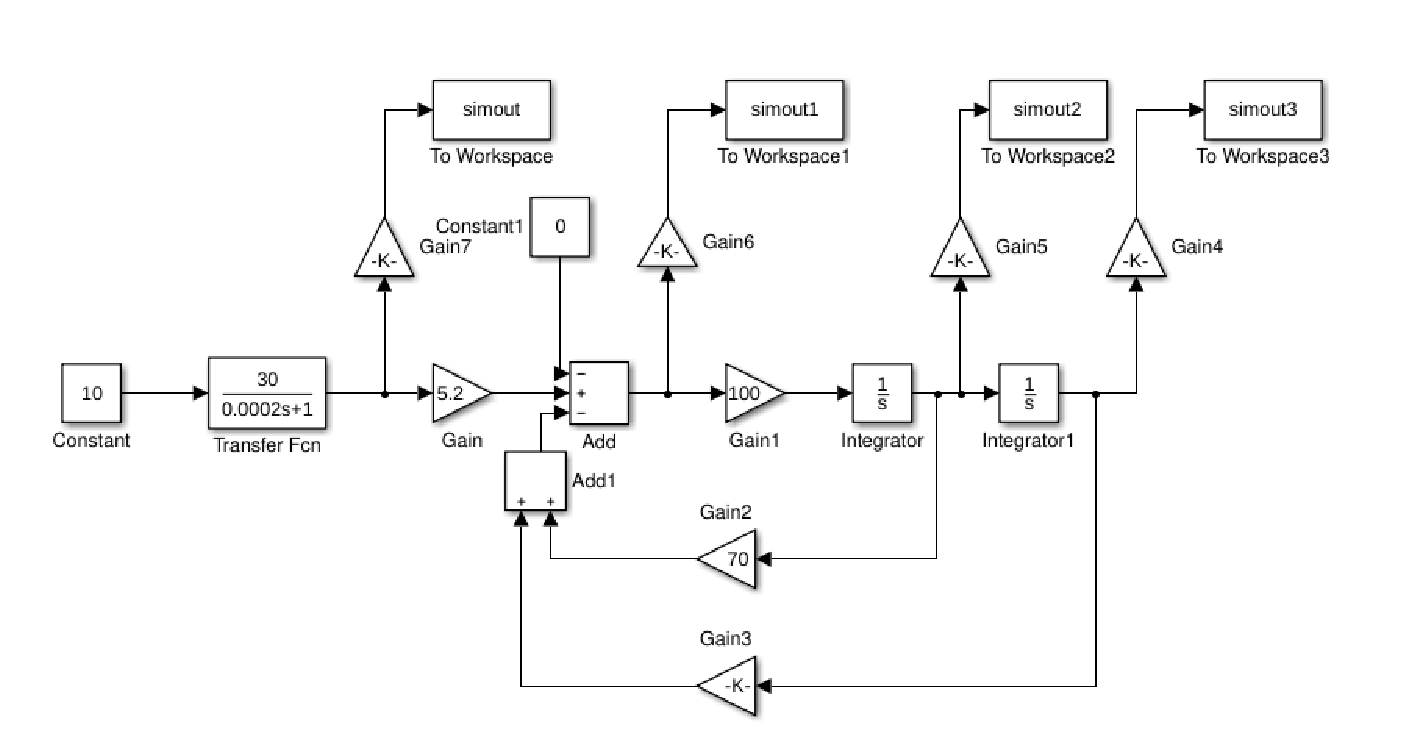
\includegraphics[width=\textwidth]{1/cxem.eps}
\caption{Cхема моделирования пьезоэлектрического исполнительного устройства}
\end{figure}
\par Выберем коэффициенты $K_{u}^{-1}$, $K_{F}$, $K_{V}$, $K_{X}$, чтобы обеспечить соответствие максимального значения измеряемого сигнала уровню 10 В на выходе измерительного устройства:
\\ $K_{u}^{-1}$=1/30
\\ $K_{F}$=0.033
\\ $K_{V}$=2.71
\\ $K_{X}$=11497.
\par На рисунках 4 -7 представлены графики переходных процессов при Fb=0 и U=10В.

\begin{figure}[H]
\centering
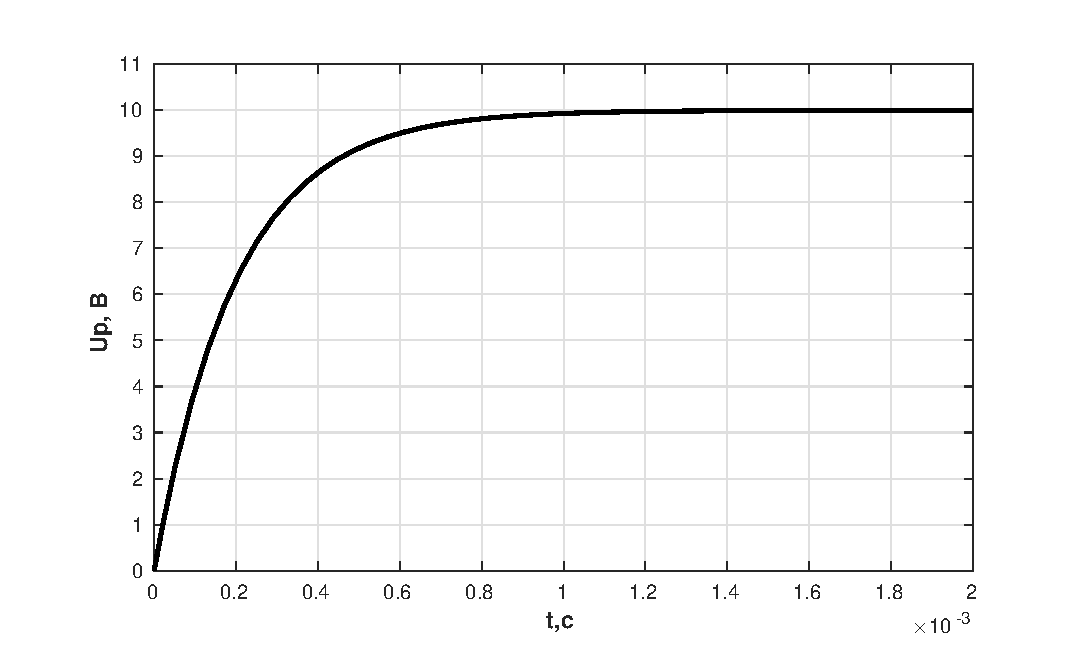
\includegraphics[width = \textwidth]{1/U1.eps}
\caption{График переходного процесса при  $F_B = 0$ и $U = 10$ B }
\end{figure}

\begin{figure}[H]
\centering
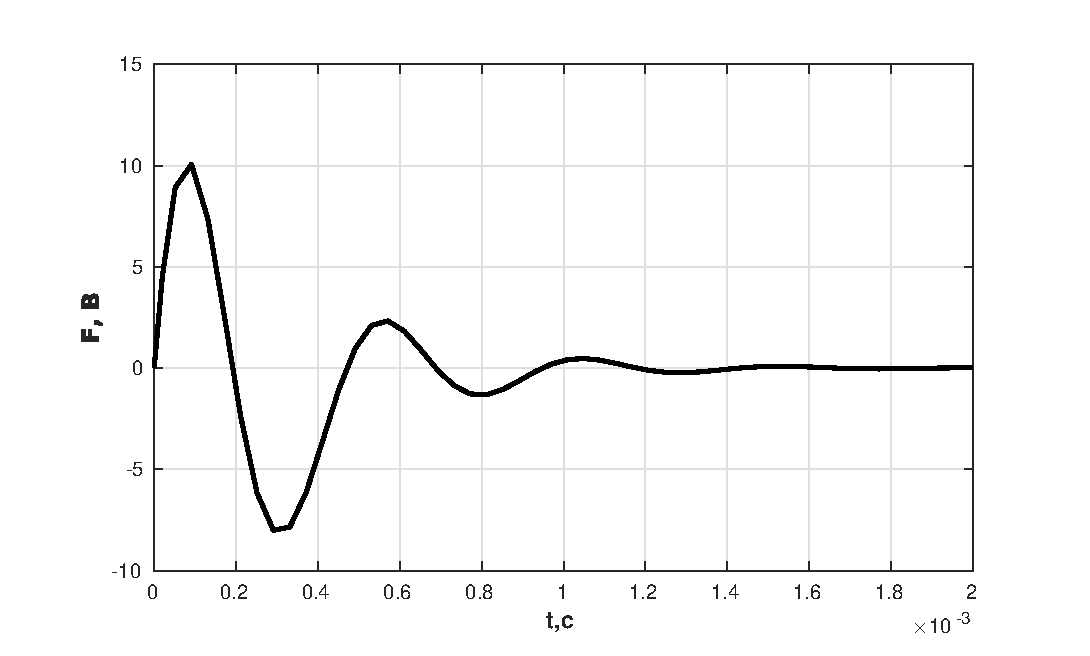
\includegraphics[width = \textwidth]{1/F1.eps}
\caption{График переходного процесса при  $F_B = 0$ и $U = 10$ B }
\end{figure}

\begin{figure}[H]
\centering
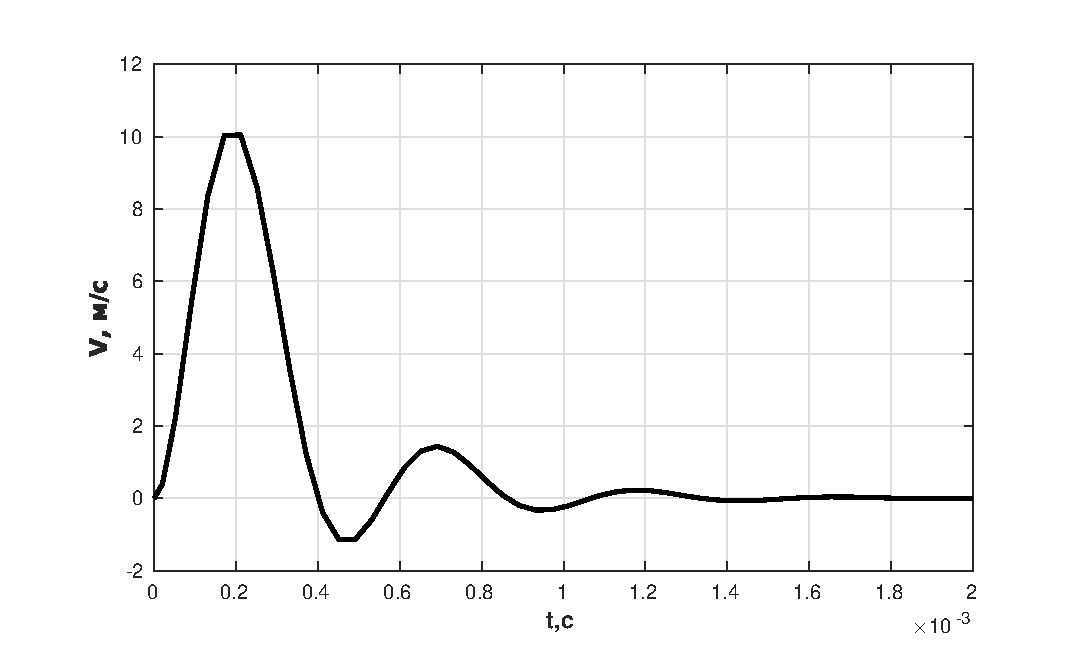
\includegraphics[width = \textwidth]{1/V1.eps}
\caption{График переходного процесса при  $F_B = 0$ и $U = 10$ B }
\end{figure}

\begin{figure}[H]
\centering
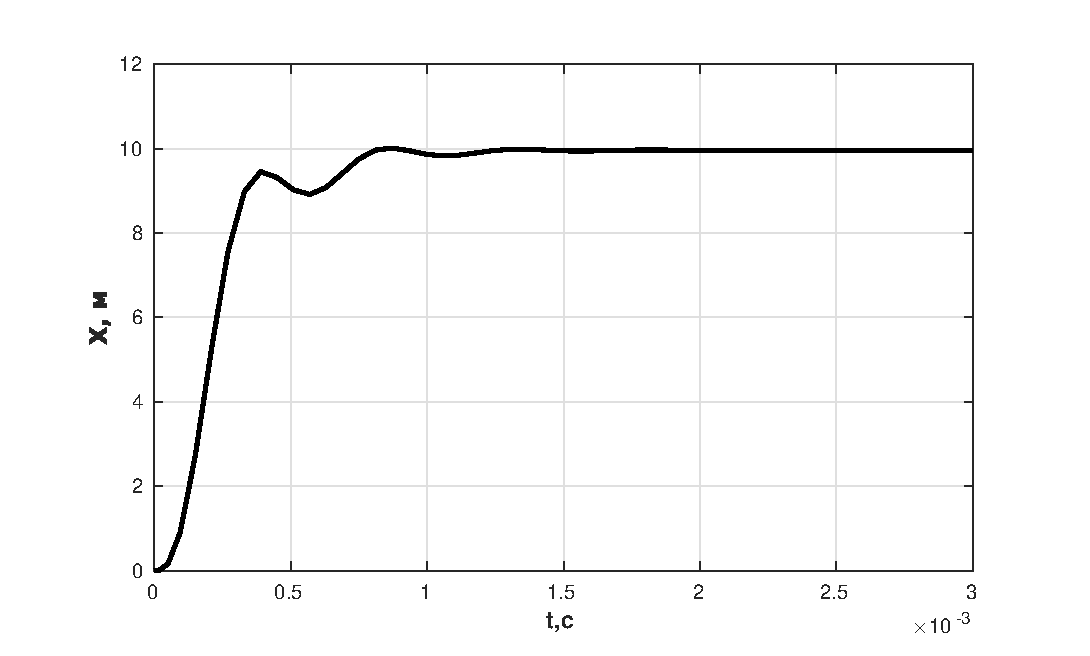
\includegraphics[width = \textwidth]{1/X1.eps}
\caption{График переходного процесса при  $F_B = 0$ и $U = 10$ B }
\end{figure}

\newpage
\begin{center}
\section{Исследование влияния массы нагрузки m на вид переходных процессов} 
\end{center}
 \par 
Диапазон изменения массы нагрузки  $\pm50\%$ от заданного значения. Будем изменять значения массы нагрузки в диапазоне от 0,005 до 0,015.
\par Графики переходных процессов представлены на рисунках 8 - 11.

\begin{figure}[H]
\centering
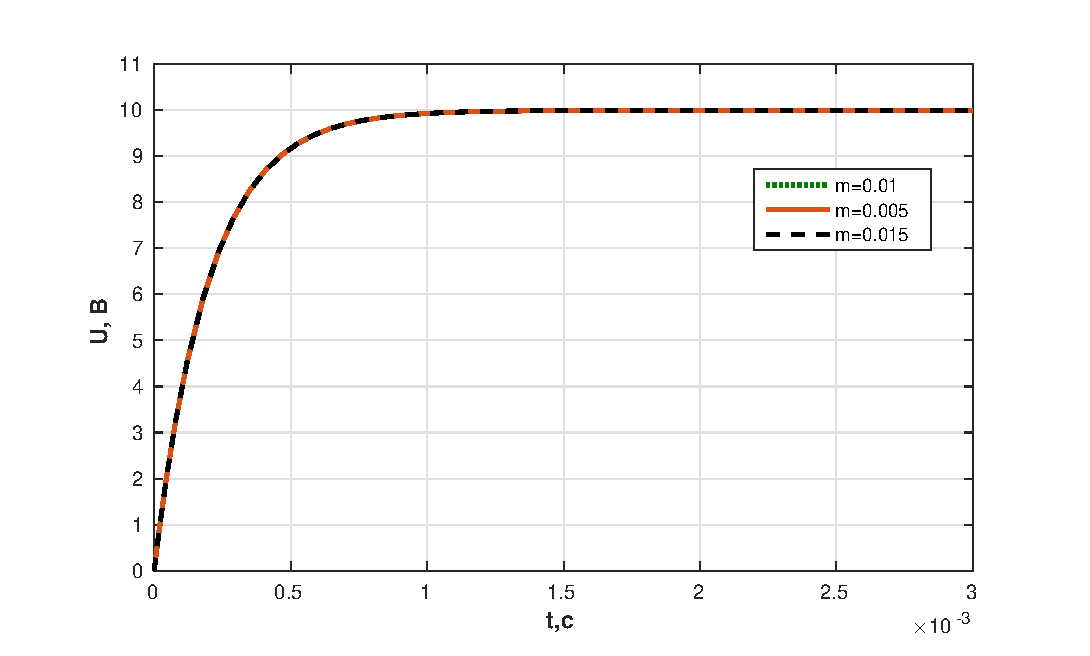
\includegraphics[width = \textwidth]{1/U2.eps}
\caption{Графики переходных процессов при различных значениях массы нагрузки}
\end{figure}

\begin{figure}[H]
\centering
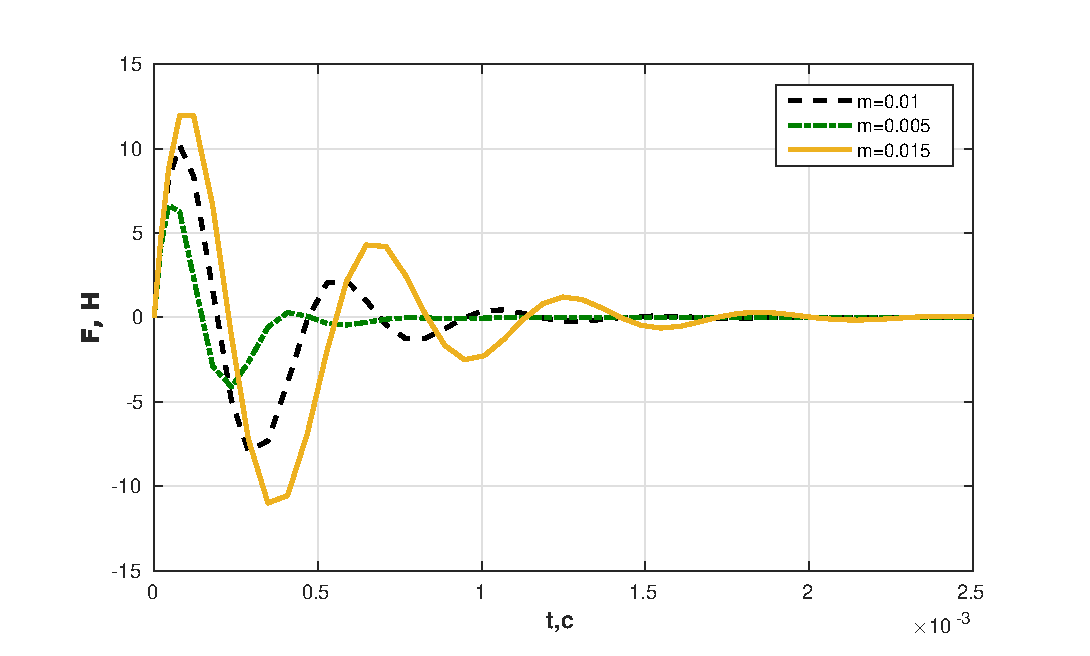
\includegraphics[width = \textwidth]{1/F2.eps}
\caption{Графики переходных процессов при различных значениях массы нагрузки}
\end{figure}

\begin{figure}[H]
\centering
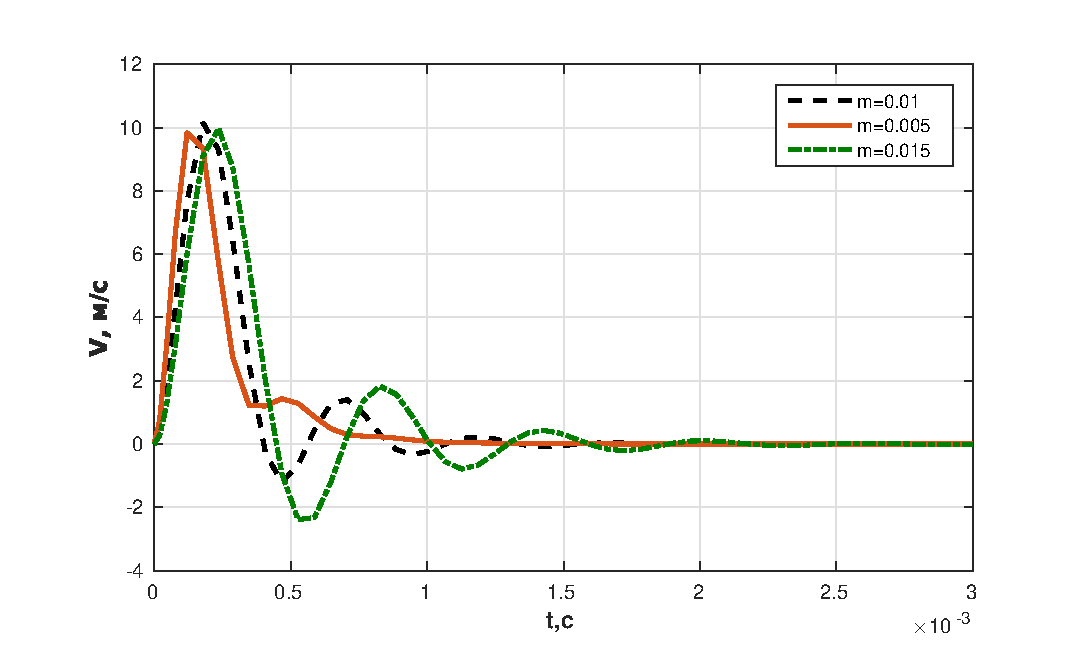
\includegraphics[width = \textwidth]{1/V2.eps}
\caption{Графики переходных процессов при различных значениях массы нагрузки}
\end{figure}

\begin{figure}[H]
\centering
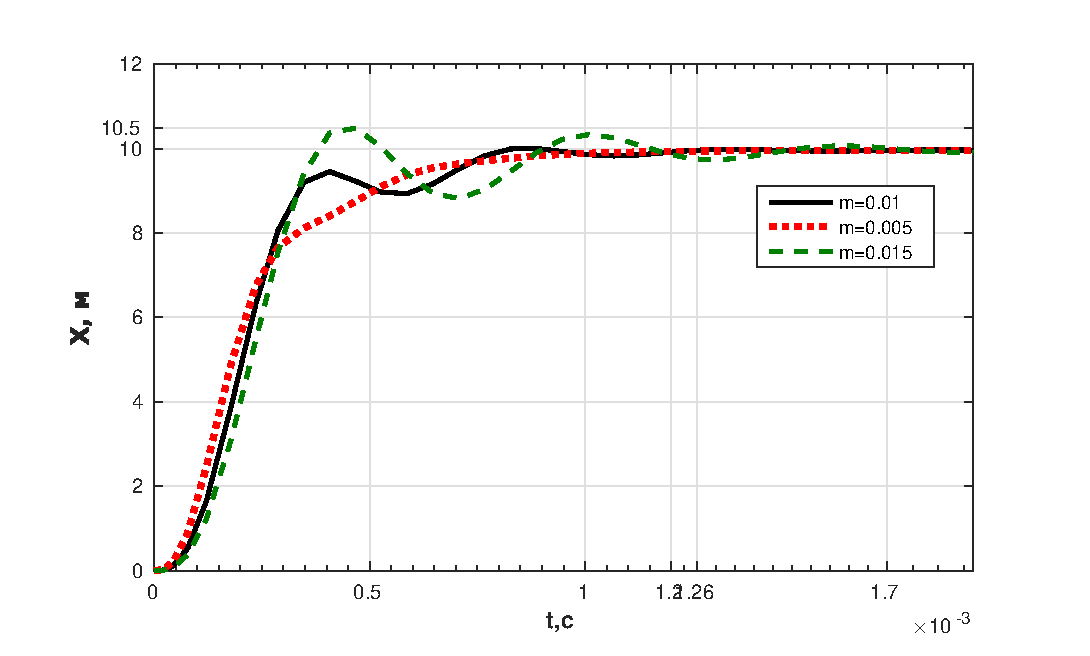
\includegraphics[width = \textwidth]{1/X2.eps}
\caption{Графики переходных процессов при различных значениях массы нагрузки}
\end{figure}
\par По графикам переходных процессов определим время переходного процесса tп, величину перерегулирования  и 
установившееся значение $x_{y}$. \par Занесем результаты в таблицу 2.

\begin{table}[h!]
\centering
\begin{threeparttable}
\caption{Характеристики системы при изменении массы нагрузки}
\renewcommand{\arraystretch}{1.8}
\begin{tabular}{ |c|c|c|c|} 
 \hline
 m,кг & tп, мс & $\sigma, \%$ & $X_{y}$  \\ 
 \hline
  0.01 & 1.26  & 0 & 10  \\ 
 \hline
 0.005 & 1.2 & 0 & 10  \\ 
 \hline
 0.015 & 1.7 & 5 & 10  \\ 
 \hline
\end{tabular}
\end{threeparttable}
\end{table}
 Величину перерегулирования принято считать по формуле:
 \begin{equation}
  \sigma=(y_{max}-y_\text{ном})/y_\text{ном}*100\%
 \end{equation}

\newpage
\begin{center}
\section{Исследование влияния $T_{u}$ на вид переходных процессов} 
\end{center}
 \par Увеличиваем исходное значение постоянной времени в 2, 4 и 6 раз. На рисунках 12 - 15 представлены графики переходных
 процессов для различных значений постоянной времени $T_{u}$.
 \begin{figure}[H]
\centering
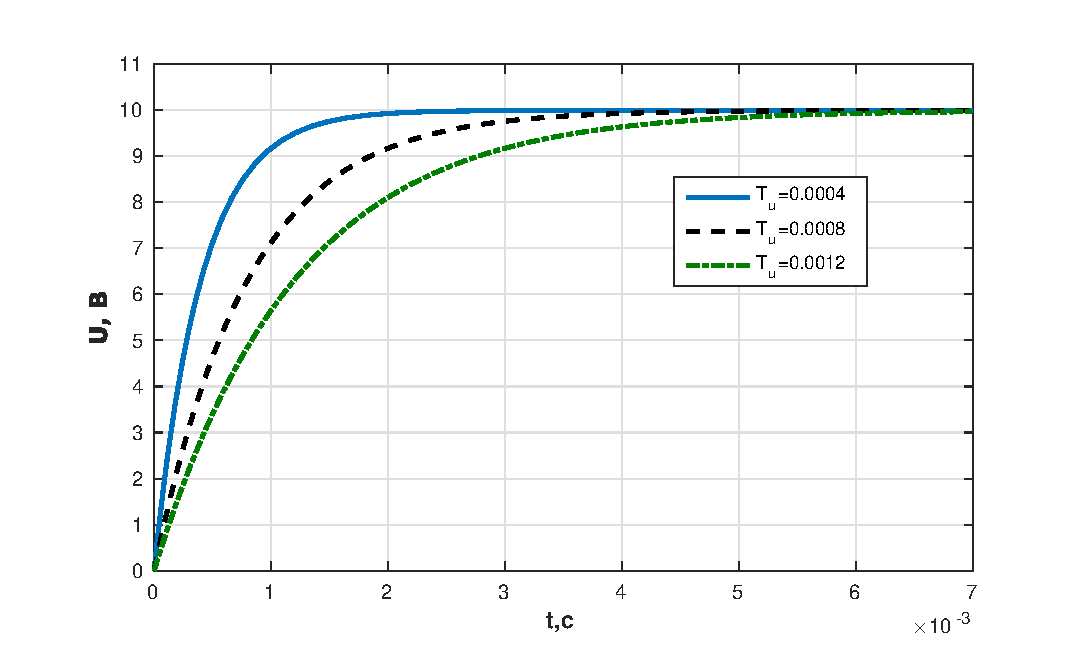
\includegraphics[width = \textwidth]{1/U3.eps}
\caption{Графики переходных процессов при различных значениях  $T_{u}$}
\end{figure}

\begin{figure}[H]
\centering
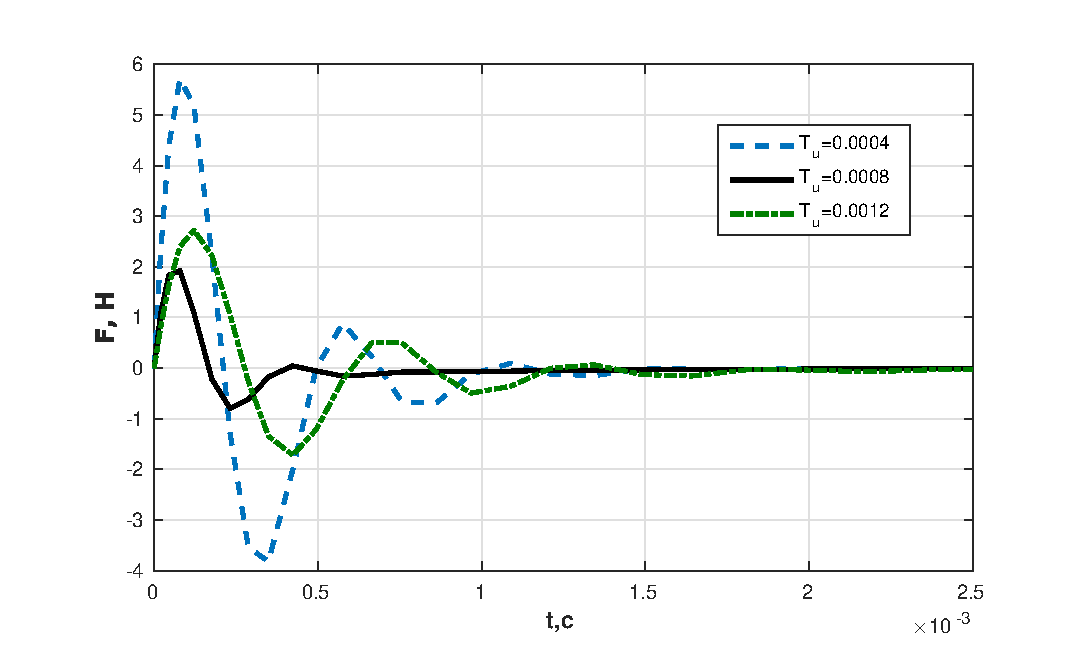
\includegraphics[width = \textwidth]{1/F3.eps}
\caption{Графики переходных процессов при различных значениях  $T_{u}$}
\end{figure}

\begin{figure}[H]
\centering
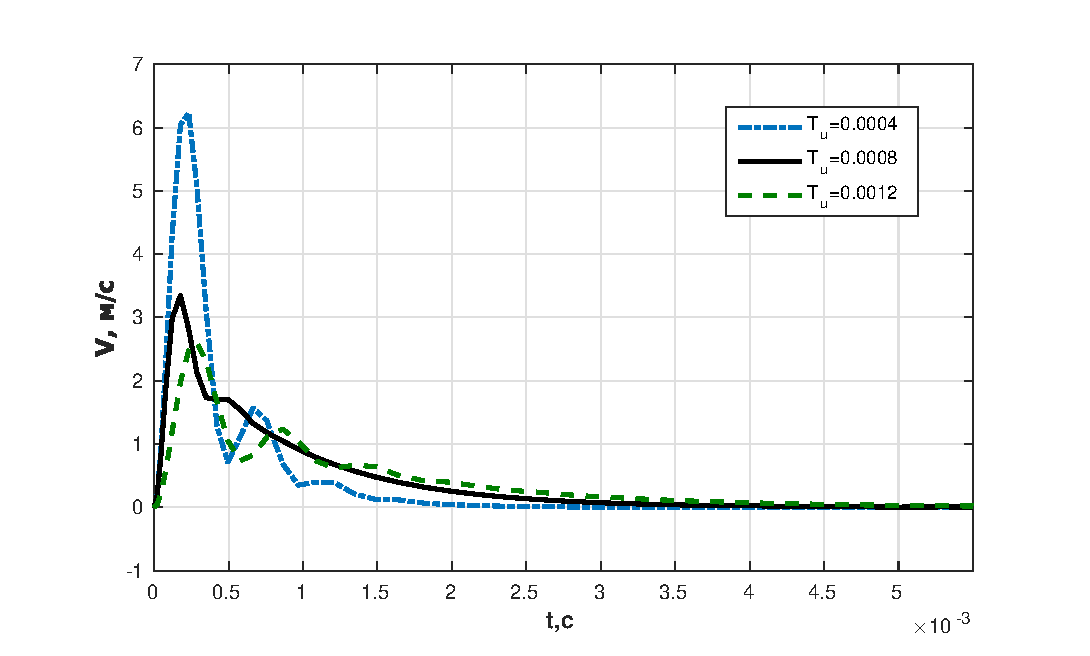
\includegraphics[width = \textwidth]{1/V3.eps}
\caption{Графики переходных процессов при различных значениях  $T_{u}$}
\end{figure}

\begin{figure}[H]
\centering
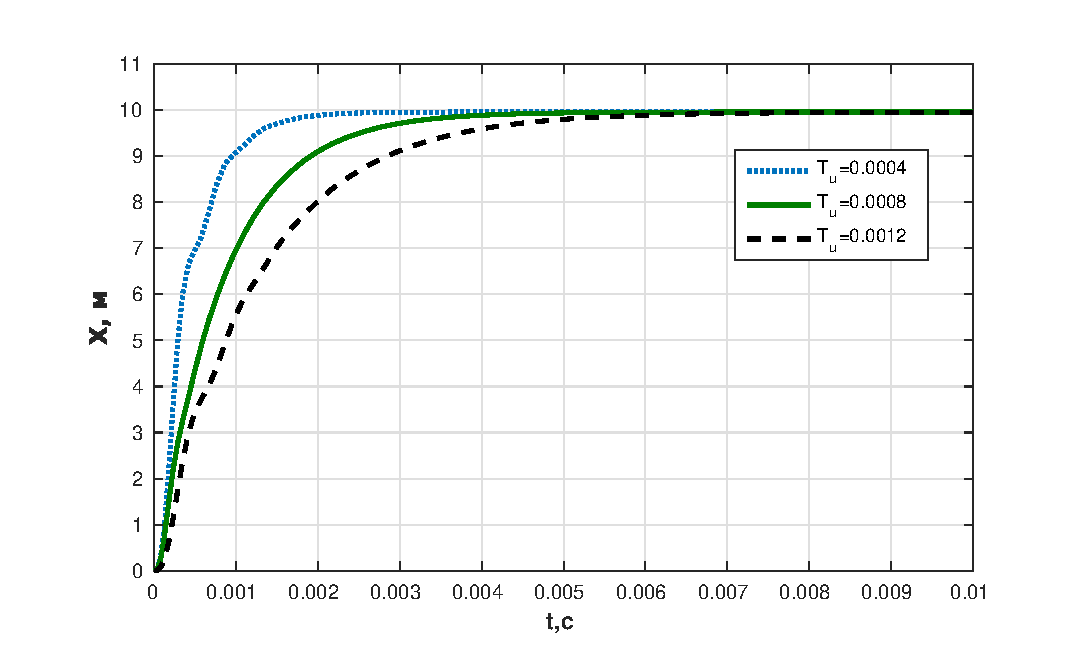
\includegraphics[width = \textwidth]{1/X3.eps}
\caption{Графики переходных процессов при различных значениях  $T_{u}$}
\end{figure}
 
\par По графикам переходных процессов определим время переходного процесса tп, величину перерегулирования  и 
установившееся значение $x_{y}$. 

\par  Необходимо составить передаточную функцию, чтобы рассчитать значения корней характеристического уравнения.
Математическая модель может быть получена на основе уравнения баланса сил в пьезодвигателе:  
\begin{equation} 
    F_y = F_O + F_\text{Д} + F_d + F_B,
    \label{F}
\end{equation}
где $F_y=C_px$ --- усилие упругой деформации ПД, $F_O=K_OU_p$ --- усилие, вызванное обратным пьезоэффектом, $F_\text{Д}=-m\displaystyle{\frac{d^2x}{dt^2}}$ --- динамическое усилие в ПД, $F_d=-K_d\displaystyle{\frac{dx}{dt}}$ --- демпфирующее усилие, обусловленное механическими потерями, $F_B$ --- внешнее воздействие, x --- перемещение, $C_p$ --- коэффициент упругости, $K_O$ --- коэффициент обратного пьезоэффекта, $U_p$ --- напряжение на электродах ПД, m --- масса перемещаемой нагрузки, $K_d$ --- коэффициент демпфирования.\par
Подставив перечисленные равенства в уравнение (\ref{F}), получим:
\begin{equation} 
    m\ddot{x} + K_d\dot{x} + C_px = K_OU_p + F_B
    \label{F1}
\end{equation}
\par Составленная по уравнению (\ref{F1}) передаточная функция будет выглядеть следующем образом:
\begin{equation} 
    W_{\text{ВУ}}(s)=\frac{K_OU_p + F_B}{ms^2 + K_ds + C_p}
    \label{FVU}
\end{equation}
\par Управление ПД осуществляется от высоковольтного усилителя, который, в нашем случае, описывается апериодическим звеном первого порядка:
\begin{equation} 
    W(s)=\frac{K_u}{T_us + 1}
\end{equation}
\par Исходя из того, что ВУ и ПД соединены последовательно, имеем передаточную следующую функцию:
\begin{equation} 
    W(s)=\frac{K_u(K_OU_p + F_B)}{(T_us + 1)(ms^2 + K_ds + C_p)}
\end{equation}
\par Найдем корни характеристического уравнения для всех сочетаний параметров и запишем все результаты в таблицу 3.

\begin{table}[h!]
\centering
\begin{threeparttable}
\caption{Характеристики системы при изменении постоянной времени}
\renewcommand{\arraystretch}{1.8}
\begin{tabular}{ |c|c|c|c|c|c|c|} 
 \hline
 $T_{u}$ & tп, с & $\sigma, \%$ & $X_{y}$ & $s_{1}$ & $s_{2}$ & $s_{3}$ \\ 
 \hline
 0.0004 & 0.0025  & 0 & 10 & -2497.69 & -3501.16-i12951 & -3501.16+i12951\\ 
 \hline
 0.0008 & 0.004 & 0 & 10 & -1248.87 & -3500.56-i12951 & -3500.56+i12951 \\ 
 \hline
 0.0012 & 0.006 & 0 & 10 & -832.59 & -3500.37-i12951 & -3500.37+i12951 \\ 
 \hline
\end{tabular}
\end{threeparttable}
\end{table} 
 
 \newpage
\begin{center}
\section{Исследование влияния коэффициента упругости Ср на вид переходных процессов} 
\end{center}
 \par
Будем проводить исcледования при $0,5C_{p}=9*10^5$ и $2C_{p}=36*10^5$.
На рисунках 16 - 17 представлены графики переходных процессов при различных значениях коэффициента упругости.
\begin{figure}[H]
\centering
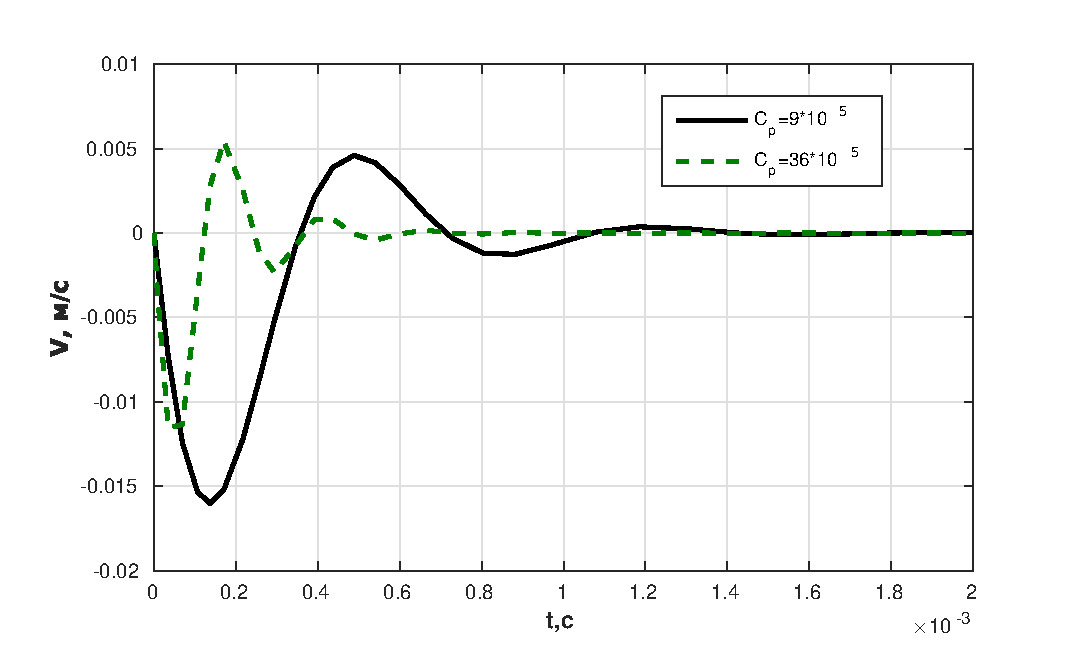
\includegraphics[width =0.8\textwidth]{1/V4.eps}
\caption{Графики переходных процессов при различных значениях  коэффициента упругости}
\end{figure}

\begin{figure}[H]
\centering
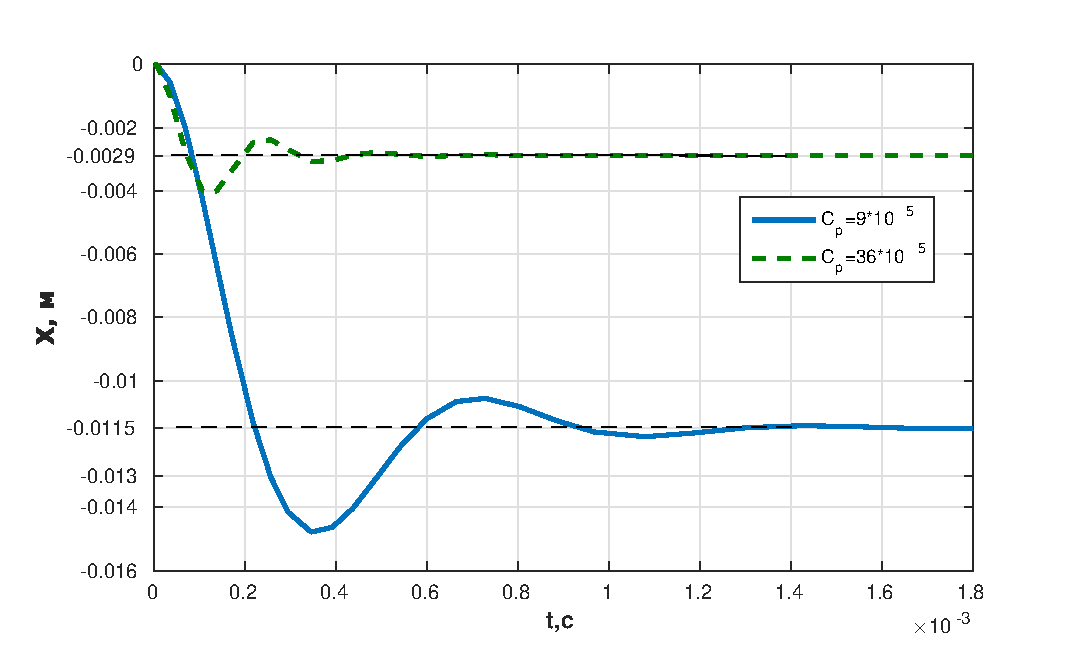
\includegraphics[width =0.8\textwidth]{1/X4.eps}
\caption{Графики переходных процессов при различных значениях коэффициента упругости}
\end{figure}
 
\newpage
\begin{center}
\section{Построение асимптотической ЛАЧХ  исполнительного устройства} 
\end{center}
 \par
 Построим асимптотическую логарифмическую характеристику для нашей системы, описываемой передаточной функцией (4). Попробуем
 представить ее в виде колебательного звена:
	\begin{equation}
	 W_\text{кз}(s) = \frac{\displaystyle{\frac{K_0}{C_p}}}{\displaystyle{\frac{m}{C_p}}s^2 + \frac{K_d}{C_p}s + 1}.
	\end{equation}
	
	Асимптотическая ЛАЧХ будет иметь нулевой наклон на уровне 
	\begin{align}
	20\lg \displaystyle{\frac{K_0}{C_p}} = 20\lg \displaystyle{\frac{5,2}{1,8\cdot10^6}} = -110,79 \text{дБ}
	\end{align}
	до сопрягающей частоты 
	\begin{align}
	\omega_c = \sqrt{\displaystyle{\frac{C_p}{m}}} = \sqrt{\displaystyle{\frac{1.8\cdot10^6}{0,01}}} = 1.3*10^4 \text{рад/с}.
	\end{align}
	После сопрягающей частоты график пойдёт под наклоном в -40 дБ/дек. 
	\par Исходя из этих утверждений асимтотическая ЛАЧХ будет выглядеть как показано на рисунке 18.
	\begin{figure}[H]
	\centering
	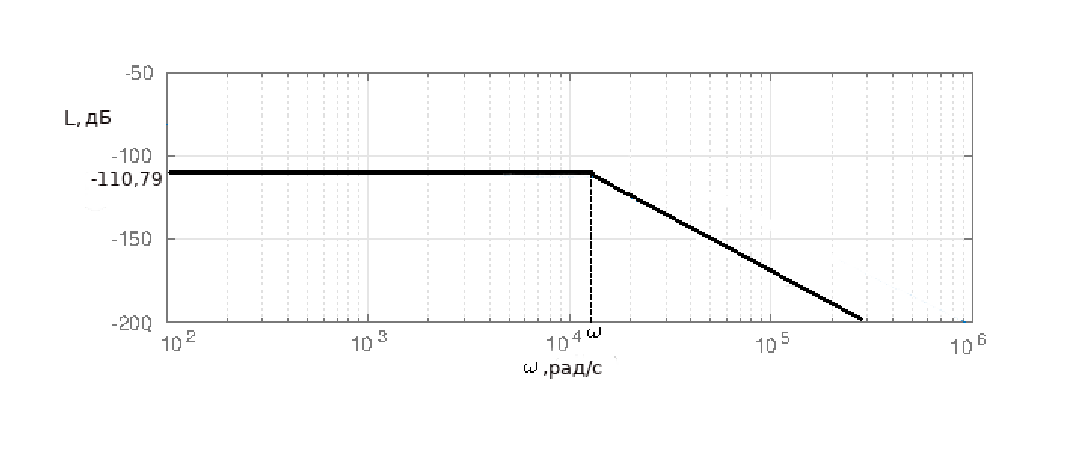
\includegraphics[width =0.8 \textwidth]{1/afchx.eps}
	\caption{Асимптотическая ЛАЧХ исполнительного устройства}
	\end{figure}
 
\newpage
\begin{center}
\section*{Вывод} 
\end{center}
 \par 
В ходе проведения данной лабораторной работы были исследованы характеристики исполнительного устройства (на 
основе пьезоэлектрического двигателя) их математические модели.
\par Были выявлены следующие закономерности при изменении постоянной времени, массы нагрузки и коэффициента упругости.
\par При увеличении значений массы нагрузки- увеличиваются значения максимального перемещения и значения сил.
При увеличении постоянной времени - уменьшаются значения силы, скорости.
При увеличении коэффициента упругости - увеличиваются максимальные значения скорости и перемещения.
\par Так же были определены: время переходного процесса, величина перерегулирования и установившееся значение перемещения.  
\end{document}
